% Longueur de référence :
%%%%%%%%%%%%%%%%%%%%%%%%%%%%%%%%%%%%%%%%%%%%%%%%%%%%%%%%%%%%%%%%%%%%%%%%%%%%%%%%%%%%%%%%%%%%%%%%%%%%%

\chapter{Les contraintes}
\label{chap:ch2}

\section{Tenseur des contraintes : définition}
    \subsection{Définition}
    \begin{wrapfigure}[7]{r}{2.5cm}
    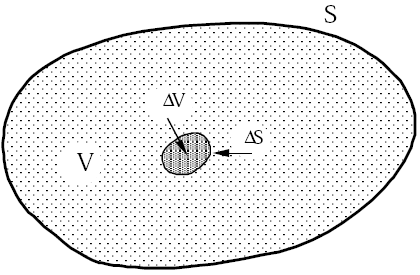
\includegraphics[scale=0.3]{ch2/image1.png}
    \captionof{figure}{Exemple considéré}
    \end{wrapfigure}
    Considérons un volume $V$ délimité par une surface fermée $S$ et considérons à l'intérieur un petit
    $\Delta V$. Quels méchants couples agissent sur lui?\\
    Il faut avant tout savoir qu'il existe trois types de contraintes
    
    \begin{enumerate}
    \item \textit{Les forces de volume} : $\vec f \Delta V$, appelées "forces à distance"). L'exemple le
    plus connu est celui de la force de pensenteur $\vec f = \rho \vec{g}$.
    \item \textit{Les couples de volume} : $\vec{\mu}\Delta V$ ne seront pas ici pris en compte. Il s'
    agit par exemple du couple créé par un champ $\vec{E}$.
    \item \textit{Les forces de surface agissant sur $\Delta S$} : il s'agit des "forces de contact", 
    elles représentent l'action du reste du volume $V$ sur l'élément $\Delta V$ isolé
    \end{enumerate}
        
        
        \subsubsection{Forces de surface agissant sur $\Delta S$}
        \begin{wrapfigure}[5]{l}{2.5cm}
        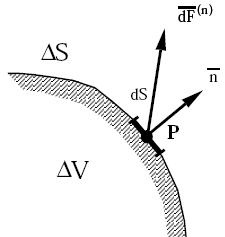
\includegraphics[scale=0.35]{ch2/image2.png}
        \captionof{figure}{Force de S.}
        \end{wrapfigure}
        Je désigne par $\overline{dF}^{(n)}$ l'action de l'extérieure sur la surface de sorte que l'
        action sur $dS$\footnote{Portion élémentaire de $dS$.} de la matière soit située du côté de 
        $\vec{n}$.\\
        On va postuler que $\overline{dF}^{(n)}$ dépend de la normale $\vec{n}$. Si je considère une 
        autre surface, j'aurai une autre normale et un vecteur $\overline{dF}^{(n)}$ différent. \\
        On \textbf{admet} que $\overline{dF}^{(n)}$ est appliquée au centre de dS.\\ \\ \\
        
    On admet également que 
    \begin{equation}
    \lim\limits_{dS \rightarrow 0} \frac{\overline{dF}^{(n)}}{dS} = \overline{T}^{(n)}
    \end{equation}
    est une fonction du point $P$ et \textbf{non} des points voisins, impliquant que le couple réparti
    en surface est nul. La dernière partie de l'égalité est le \textit{vecteur contrainte, au point 
    $P$, associé à la facette\footnote{Petite surface.} de normale $\vec{n}$.}\\
    La force dépend bien de $\vec{n}$ mais durant les secondaires celle-ci était toujours parallèle à
    $\vec{n}$ ce qui ne sera plus forcément le cas ici.

    \subsection{La loi de Cauchy}
    \begin{wrapfigure}[12]{l}{6cm}
    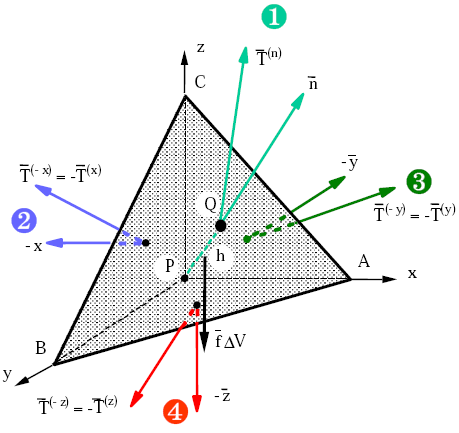
\includegraphics[scale=0.45]{ch2/image3.png}
    \captionof{figure}{Loi de Cauchy}
    \end{wrapfigure}
    Considérons un tétraèdre élémentaire $PABC$ dont les arêtes sont alignées selon les axes $x,y,z$
    et la face est de normale $\vec{n} $. Afin de dériver cette loi, je regarde le vecteur contrainte
    associé à $\vec n$ (Derrière la contrainte, il y a donc un tenseur d'ordre 2). Comme la contrainte
    est une force par surface, je dois calculer les surfaces correspondantes. Récapitulons :
    \begin{enumerate}
    \item \textit{Face ABC} : normale $\vec{n} $\ \ \ contrainte : $\overline{T}^{(n)}$
    \item \textit{Face PBC} : normale -$\vec{x} $\ \  contrainte : $\overline{T}^{(-x)} = -\overline{T}^{(x)}$
    \item \textit{Face PCA} : normale -$\vec{y} $\ \  contrainte : $\overline{T}^{(-y)} = -\overline{T}^{(y)}$
    \item \textit{Face PAB} : normale -$\vec{z} $\ \  contrainte : $\overline{T}^{(-z)} = -\overline{T}^{(z)}$
    \end{enumerate}\ \\ 
    Chaque surface vaut alors
    \begin{enumerate}
    \item \textit{Face ABC} : aire =  $\Delta S$\ \ (Par hypothèse)
    \item \textit{Face PBC} : aire =  $\Delta S\cos(\vec{n},\vec{x}) = \Delta S n_x$
    \item \textit{Face PCA} : aire =  $\Delta S\cos(\vec{n},\vec{y}) = \Delta S n_y$
    \item \textit{Face PAB} : aire =  $\Delta S\cos(\vec{n},\vec{z}) = \Delta S n_z$
    \end{enumerate}
    
    En appliquant la loi de la résultante cinétique\footnote{$\frac{d\vec{R}}{dt} = \sum \vec{F_e}$} au volume 
    élémentaire du tétraèdre, on obtiens 
    \begin{equation}
    \left[\rho\vec{v}\left(\dfrac{1}{3}h\Delta S\right)\right]^{\bullet} = \vec{f}\left(\dfrac{1}{3}h\Delta S\right) +
    \underbrace{\overline{T}^{(n)}\Delta S}_{1} + \underbrace{\overline{T}^{(-x)}\Delta S_x}_{2} + 
    \underbrace{\overline{T}^{(-y)}\Delta S_y}_{3} + \underbrace{\overline{T}^{(-z)}\Delta S_z}_{4}
    \end{equation}
    ou enocre
    \begin{equation}
    \left[\rho\vec{v}\left(\dfrac{1}{3}h\Delta S\right)\right]^{\bullet} -\vec{f}\left(\dfrac{1}{3}h\Delta S\right)
    = \left[\overline{T}^{(n)}+\overline{T}^{(-x)}n_x + \overline{T}^{(-y)}n_y
    + \overline{T}^{(-z)}n_z\right]\Delta S
    \end{equation}
    En effectuant $\Delta S \rightarrow 0$ (en faisant tendre $h$ vers 0) il reste
    \begin{equation}
    0 = \left[\overline{T}^{(n)}+\overline{T}^{(-x)}n_x +\overline{T}^{(-y)}n_y+\overline{T}^{(-z)}n_z\right]
    \Delta S
    \end{equation}
    Ce qui donne\\
    
    \prop{\textsc{Loi de Cauchy}
    \begin{equation}
    \overline{T}^{(n)} = \overline{T}^{(x)}n_x + \overline{T}^{(y)}n_y+ \overline{T}^{(z)}n_z
    \end{equation}}
    Cette loi montre un qu'un vecteur est associé à toute direction par une combili des consinus directeur de
    cette direction : il s'agit d'un tenseur !
    
    \subsection{Le tenseur des contraintes}
    En projetant les vecteurs $\overline{T}^{(x)}, \overline{T}^{(y)}$ et $\overline{T}^{(z)}$ sur les axes de
    coordonnés et en appelant $\tau_{ij}$ la composante selon l'axe $j$ du vecteur contrainte agissant sur la 
    facette normale $i$ on obtient la \textbf{relation de Cauchy}
    \begin{equation}
    T_j^{(n)} = \tau_{ij}n_i
    \end{equation}
    où $\tau_{ij}$ sont les composantes d'un tenseur du second ordre : le \textbf{tenseur des contraites}.
    
    \newpage
    Par exemple, si $\vec{n} \parallel \vec{1_x}_{1} : \vec{n} = (1,0,0) \rightarrow  \overline{T}^{(n)} =
     \overline{T}_1 =  \overline{T}^{(1)}$. Cela montre que $ \overline{T}^{(i)}$ est le vecteur contrainte
     agissant sur la facette de normale $x_i$.\\
     
     Les valeurs de $\tau_{ij}$ sont les 9 composantes du tenseur des contraintes : l'indice $i$ représente
     la normale à la facette considérée et l'indice $j$ la direction sur laquelle on projette la contrainte
     correspondant à cette facette. Un peu de vocabulaire à présent :
     \begin{itemize}
     \item Lorsque deux indices sont égaux : \textit{composante normale} notée $\sigma$.
     \item Lorsque deux indices sont différents : \textit{composante tangentielle}.
     \end{itemize}
    
    
    
    
\section{La dérivée matérielle}
    \subsection{Définition}
    La dérivée matérielle est la dérivée par rapport au temps, prise en suivant la particule dans son 
    mouvement (par exemple, le calcul de l'accélération de ta merco). Si une particule est en $\vec{x}$
    à l'instant $t$ et en $\vec{x}'$ en $t+dt$, on a par définition
    \begin{equation}
    T_{k\ l\dots}^\bullet = \lim\limits_{dt \rightarrow 0} \dfrac{T_{k\ l\dots}(\vec{x}',t+dt) - T_{k\ l\dots}
    (\vec x,t)}{dt}
    \end{equation}
    
    \subsection{Dérivée matérielle d'une grandeur locale}
    La position $\vec{x}$ dépend de $t \rightarrow T_{kl\dots} (\vec{x},t)$. Dès lors
    \begin{equation}
    T_{k\ l\dots}^\bullet = \frac{\partial T_{k\ l\dots}}{\partial t} + \frac{T_{k\ l\dots}}{\partial x_i}
    \frac{dx_i}{dt}\ \ \ \ \text{avec}\ \left\{\begin{array}{ll}
    \partial_0 &= \frac{\partial}{\partial t}  \\
    v_i &= \frac{dx_i}{dt} 
    \end{array}\right.
    \end{equation}
    Ce qui nous donne 
    \begin{equation}
    T_{k\ l\dots}^\bullet = \partial_0T_{k\ l\dots} + v_i.\partial_iT_{k\ l\dots} = T_{k\ l\dots}^\bullet = \partial_0T_{k\ l\dots} +
    (\vec v.\overline{grad})T_{k\ l\dots}
    \end{equation}
    
    \subsection{Dérivée matérielle d'une intégrale de volume}
    La "démonstrations" des différentes formules est très calculatoire. On obtient trois équations pour une
    même dérivée qu'il faudra utiliser selon le contexte
    \begin{equation}
    \left\{\begin{array}{ll}
    I^\bullet &= \int_V \partial_0 T_{k\ l\dots} dV + \oint_S T_{k\ l\dots} v_in_i dS\\
    I^\bullet &= \int_V [\partial_0T_{k\ l\dots} + \partial_i(v_iT_{k\ l\dots})]\ dV\\
    I^\bullet &= [T_{k\ l\dots}^\bullet + T_{k\ l\dots}(\partial_iv_i)]dV
    \end{array}\right.
    \end{equation}
    
    
    
\section{Les lois fondamentales}
    Il existe trois grandes lois de "conversation" ou "bilan" : la conservation de la masse, de la 
    résultante cinétique et du moment cinétique.
    
    \subsection{Conservation de la masse} 
    Soit un volume $V$ de masse $M$ t.q. $M = \int_V \rho dV$. La masse est onstante dans le temps, sa 
    dérivée matérielle est forcément nulle. La dérivée matérielle d'une intégrale de volume étant : $I^
    \bullet = \int_V [\partial_0T_{k\ l\dots} + \partial_i(v_iT_{k\ l\dots})]\ dV$, on trouve :
    \begin{equation}
    \dot{M} = \int_V [\partial_0\rho + \partial_i(v_i\rho)]dV = 0
    \end{equation}
    On trouve alors l'équation locale de conservation de la masse\footnote{Remarquons que $\rho$ se trouve
    dans l'expression de la dérivée, c'est parce que ce n'est pas forcément une constante.}, l'\textit{équation 
    de continuité :}
    \prop{\textsc{Équation de continuité de la masse}\begin{equation}
    \partial_0\rho + \partial_i(v_i\rho) = 0
    \end{equation}
    Plusieurs forme peuvent exister, car 
    \begin{equation}
    \frac{d\rho}{dt} = \frac{\partial \rho}{\partial t} + \frac{\partial \rho}{\partial x_i}v_i
    \end{equation}}\ \\
    \begin{wrapfigure}[8]{r}{3cm}
    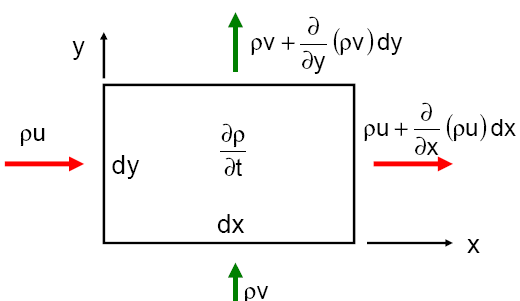
\includegraphics[scale=0.3]{ch2/image4.png}
    \captionof{figure}{Conservation de la masse}
    \end{wrapfigure}
    On retrouve facilement cette conservation sur un rectangle élémentaire ; comme cette loi doit être vrai
    pour tout volume, cela concerne aussi ce rectangle. La variation de masse au cours du temps c'est la masse qui
    rentre à laquelle on soustrait la masse qui sort (tronqué au premier ordre). En faisant de même sur les
    deux autres face :
    \begin{equation}
    \frac{d\rho}{dt}dxdy = \rho u du + \rho v dx - \left( \rho u + \frac{\partial}{\partial x}(\rho u)dx\right)
    dy - \left( \rho v + \frac{\partial}{\partial x}(\rho v)dy\right)dx
    \end{equation}
    Après simplification, on retrouve le St-Graal :
    \begin{equation}
    \frac{\partial \rho}{\partial t} + \frac{\partial}{\partial x}(\rho u) + \frac{\partial}{\partial y}(\rho v) = 0
    \end{equation}
    
    Ceci a des conséquence pour le calcul de la dérivée matériel d'une intégrale de volume. Comme $I = \int_V
    T\dots \rho dV = \int_M T\dots dM$, on trouve :
    \begin{equation}
    \dot{I} = \underbrace{\int_M \dot{T}\dots dM}_{1} = \underbrace{\int_V \dot{T}\dots\rho dV}_{2}
    \end{equation}
    \begin{enumerate}
    \item On peut dériver sous l'intégrale car la masse est constante.
    \item On peut dériver sous l'intégrale en groupant $\rho dV$.
    \end{enumerate}
    
    \subsection{Loi de la résultance cinétique}
    Par définition, $\overline{\mathcal{R}} = \int_V \vec{v}.dM = \int_V \vec{v}.\rho\ dV$? On a donc de 
    façon directe :
    \begin{equation}
    \dot{\overline{\mathcal{R}}} = \int_V \dot{\vec{v}}.\rho\ dV
    \end{equation}
    et la loi de la résultante cinétique (\textit{Cf. Mécanique Rationnelle II}) s'écrit en égalant à cette
    expressions les différentes forces externes, à savoir de volume et de surface :
    \begin{equation}
    \int_V \rho \dot{v_i}\ dV = \int_V f_i\ dV + \oint_S T_i^{(n)}\ dS
    \end{equation}
    Par application de la \textit{loi de Cauchy} $T_i^{(n)} = \tau_{ji}n_j$ suivi de la loi de Gauss :
    \begin{equation}
    \oint_S T_i^{(n)}\ dS = \int_V \partial_j \tau_{ji}\ dV
    \end{equation}
    On à donc :
    \begin{equation}
    \int_V \rho \dot{v_i}\ dV = \int_V [f_i +\partial_j \tau_{ji}]\ dV
    \end{equation}
    On peut en déduire les trois équations de mouvements : \\
    \prop{\textsc{Équations du mouvement (dynamique)} :
    \begin{equation}
    \rho[\partial_0v_i + v_k\partial_kv_i] = f_i + \partial_j\tau_{ji}
    \end{equation}
    où le premier membre est nul si l'on se trouve à l'\textbf{équilibre de translation} (statique) :
    \begin{equation}
     f_i + \tau_{ji,j} = 0
    \end{equation}}\ \\
    
    \subsection{Loi du moment cinétique}
    \textit{"C'est le plus chiant à faire"}. Pour y aller simplement, je prends un poin géométrique par
    rapport auquel je prends tous mes moments : \textit{bras de levier} $\times \vec{r}$. Par définition:
    \begin{equation}
    \overline{\mathcal{M}} = \int_M (\vec{r}\times\vec{v}).\rho\ dV
    \end{equation}
    On a donc directement :
    \begin{equation}
    \dot{\overline{\mathcal{M}}} = \int_M (\vec{r}\times\vec{v})^\bullet.\rho\ dV
    \end{equation}
    ou :
    \begin{equation}
    \dot{\overline{\mathcal{M}}} = \int_M \underbrace{[(\vec{v}\times\vec{v})]}_{\vec{0}} + (\vec{r}
    \times \vec{v}^\bullet]\rho\ dV
    \end{equation}
    On trouve alors la fameuse loi :\\
    
    \prop{\textsc{Loi du moment cinétique} :
    \begin{equation}
    \int_V \underbrace{(\vec{r}\times \dot{\vec{v}})\rho\ dV}_{1} = \underbrace{\int_V (\vec{r}\times\vec{f})\
    dV}_{2} + \underbrace{\oint_S (\vec{r} \times \overline{T}^{(n)})\ dS}_{3}
    \end{equation}
    \begin{enumerate}
    \item Dérivée du moment cinétique
    \item Moment des forces de volume
    \item Moment des forces de surface
    \end{enumerate}}\ \\
    
    En essayant de nettoyer cette expression (relation de Cauchy puis Gauss, simplification des dérivées par
    symbole de Kronecker, ...) on trouve finalement la relation\footnote{Cf. slide 43-48.}
    \begin{equation}
    \tau_{jk} = \tau_{kj}
    \end{equation}
    impliquant l'équilibre de rotation\footnote{Aussi bien valide en statique qu'en dynamique.}.
    
    
    \subsection{Théorème de Cauchy - Poisson}
    Ce double théorème lie les équations d'équilibres en volume et en surface avec les lois de la résultante 
    et du moment cinétique.\\
    \prop{\textsc{Théorème de Cauchy - Poisson}
    \begin{equation}
    T_j^{(n)} = \tau_{ij}n_i\ \ \ \ \ \ \rho \dot{v}_i = \tau_{ij,j} + f_i\ \ \ \ \ \ \tau_{ij} = \tau_{ji}
    \end{equation}}


\section{Valeurs principales et directions principales}
Cette section va donner réponse aux deux questions suivantes, concernant les proriétés du tenseur des
contraintes : 
\begin{enumerate}
\item Existe-t-il des directions pour lesquelles le vecteur contrainte est alligné selon la normale ?
\item Existe-t-il des directions pour lesquelles la composante normale du vecteur contrainte est extrémum?
\end{enumerate}

    \subsection{Valeurs propres et directions principales}
    \begin{wrapfigure}[11]{r}{3cm}
    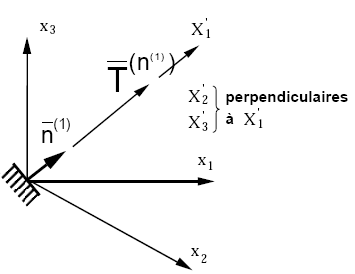
\includegraphics[scale=0.5]{ch2/image6.png}
    \captionof{figure}{$\vec{n}// \overline{T}^{(n)}$}
    \end{wrapfigure}
    Occupons nous de la première question. Le vecteur des contrainte est alligné selon la normale si 
    $\overline{T}^{(n)} = \lambda \overline{n}$, c'est à dire si :
    \begin{equation}
    \tau_{ij}n_j = \lambda n_i
    \end{equation}
    Après réorganisation, on trouve $(\tau_{ij} - \lambda \delta_{ij}) = 0$ ; il s'agit d'un système
    algébrique dont les inconnus sont $n_j$. La solution triviale n'est pas accepté, $\vec{n}$ étant 
    unitaire. On doit donc avoir : 
    \begin{equation}
    \text{det}|\tau_{ij} - \lambda \delta_{ij}|=0 \Leftrightarrow \left|\begin{array}{ccc}
    \sigma_x - \lambda      &\tau_{xy}              &\tau_{xz}\\
    \tau_{xy}               &\sigma_y-\lambda       &\tau_{yz}\\
    \tau_{xz}               &\tau_{yz}              &\sigma_z - \lambda
    \end{array}\right| = 0
    \end{equation}
    Ceci donne lieu à une équation du $3^e$ degré $\rightarrow$ il y a au moins une racine réelle ($\lambda_1$). 
    Pour cette racine, le système est compatible et il y a au moins une solution, notée $\overline{n}^{(1)}$.
    Qu'en est-il des deux autres ?\\
    Effectuons un changement de repère : $\{x_1,x_2,x_3\}\rightarrow \{X_1',X_2',X_3'\}$ tel que 
    $X_2'$ et $X_3'$ soient $\perp$ à $X_1'$. Le changement d'axe s'effectue grace à $\tau_{PQ}' = \alpha_{Pi}
    \alpha_{Qj}\tau_{ij}$. On obtient (avec $\tau_{12}' = \tau_{13}' = 0$ car $X_1' // n^{(1)}$) :
    \begin{equation}
    \left|\begin{array}{ccc}
    \sigma_x - \lambda      &0                      &0 \\
    0                       &\sigma_y'-\lambda       &\tau_{yz}'\\
    0                       &\tau_{yz}'              &\sigma_z' - \lambda
    \end{array}\right| = 0
    \end{equation}
    La calcul du déterminant fait apparaître un polynôme du second ordre dont le discriminant est toujours
    positif ou nul $\rightarrow \lambda_2$ et $\lambda_3$ sont aussi réelle. Nos trois racines sont ainsi
    réelles, ce qui permet de répondre à la question initiale en énonçant la propriété :\\
    
    \prop{\begin{enumerate}
    \item Il existe au moins trois directions pour lesquelles $\overline{n} // \overline{T}^{(n)}$
    \item Les directions $\overline{n}^{(1)}$ et $\overline{n}^{(2)}$ correspondant à $\lambda_1 \neq
    \lambda_2$ sont orthogonales.
    \item Les directions $\overline{n}^{(1)}$ et $\overline{n}^{(2)}$ correspondant à $\lambda_1 =
    \lambda_2 = \lambda^*$ définissent un plan où toutes les directions sont principales.
    \end{enumerate}}\ \\
    $\Rightarrow$ \textbf{toutes} les directions du plan $\overline{n}^{(1)}\ \overline{n}^{(2)}$ sont donc
    principales et on peut y \textbf{choisir} deux directions orthogonales, ce qui généralise la propriété.
    
    
    \subsection{Propriétés du tenseur des contraintes}
    Répondons maintenant à la deuxième question. Soit la composante perpendiculaire $\sigma_n 
    = \overline{T}^{(n)}.\overline{n}$, ce qui peut s'expliciter :
    \begin{equation}
    \sigma_n = \tau_{ij}n_jn_i
    \end{equation}
    Il s'agit d'un extrémum lié par la condition $n_in_j=1$. On peut le rendre libre à l'aide des 
    multiplicateur de Lagrange :
    \begin{equation}
    (\tau_{ij}n_j)n_i - \lambda (n_in_i - 1)
    \end{equation}
    Afin de (trouver l'extremum ?), dérivons notre expressions et égalons la à zéro :
    \begin{equation}
    \frac{\partial}{\partial n_k}[(\tau_{ij}n_j)n_i - \lambda (n_in_i - 1)] = 0
    \end{equation}
    On remarque que $\frac{\partial n_i}{n_1} = 1$ si $i=1$ et 0 sinon. On peut donc dire que 
    $\frac{\partial n_i}{\partial n_k} = \delta_{ik}$, ce qui donne 
    \begin{equation}
    \tau_{ij}n_j\delta_{ik} + \tau_{ij}n_i \delta_{jk} - 2\lambda n_i \delta_{ik} = 0
    \end{equation}
    Ou encore:
    \begin{equation}
    \tau_{ij}n_j + \tau_{ij}n_i - 2\lambda n_i  = 0
    \end{equation}
    Après ménage, on trouve les vecteurs propres du problème. Pour le tenseur des contraintes, on appelle
    ça les \textit{directions principales :}
    \begin{equation}
    (\tau_{kj} - \lambda\delta_{kj})n_j = 0
    \end{equation}
    
    Nous avons jusqu'ici travaillé sur des vecteurs. Par extension, de tout tenseur symétrique du second
    ordre :\\
    
    \prop{\textsc{Le tenseur des contraintes :}
    \begin{itemize}
    \item Possède trois directions principales (au moins 3)
    \item Ces directions sont orthogonales
    \item Les valeurs principales sont les contraintes principales (les contraintes normales selon ces
    directions)
    \item Pour ces directions, la contrainte normale est extrémum
    \end{itemize}}
    
        \subsubsection{Invariants du tenseur des contraintes}
        On peut définir trois invariants :
        \begin{equation}
        \left\{\begin{array}{ll}
        I_1 &= \tau_{ii} \\
        I_2 &= \frac{1}{2} (\tau_{ij}\tau_{ji} - \tau_{ii}\tau_{jj})\\
        I_3 &= \frac{1}{6}\delta_{pqr}\delta_{ijk}\tau_{pi}\tau_{qj}\tau_{rk}
        \end{array}\right.
        \end{equation}
        Ceux-ci amènent l'équation caractéristique sous la forme :
        \begin{equation}
        \lambda^3 = I_1 \lambda^2 + I_2 \lambda + I_3
        \end{equation}
        Le Th. Hamilton-Cayley démontre que tous les invariants d'ordre supérieurs s'expriment en fonction
        de ceux-ci.
    

\section{Changement d'axes : cercle de Mohr}
    \subsection{Construction du cercle de Mohr}
    Il s'agit d'une \textit{construction graphique} traduisant les lois de changement d'axes pour les 
    composantes du tenseur en un point. Il permet :
    \begin{itemize}
    \item de trouver les composantes du tenseur des contraintes, pour 'importe quelle orientation de
    normale (de facette)
    \item de trouver les valeurs des contraintes principales et les  directions correspondantes
    \item de trouver les valeurs des contraintes tangentielles extrémum et les directions 
    correspondantes
    \item de vérifier rapidement des résultats obtenus par calculs
    \end{itemize}
    
    \begin{wrapfigure}[7]{l}{4cm}
    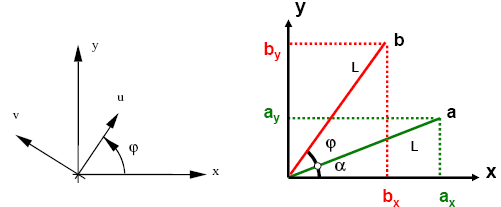
\includegraphics[scale=0.3]{ch2/image7.png}
    \captionof{figure}{Rotation d'axes}
    \end{wrapfigure}
    Pour obtenir le cercle de Mohr, le point de départ est la formule de changement d'axe appliquée à une
    rotation d'angle $\varphi$ autour de l'axe $z$, dans le sens trigonométrique. En distribuant termes à
    termes, on peut faire apparaître un facteur $2\phi$\footnote{Il faut appliquer la définition de 
    $\tau_{ij}$, exprimer les $2\phi$, ... Rien de compliqué, mais fastidieux.} :
    \begin{equation}
    \left\{\begin{array}{ll}
    \sigma_u &=  \dfrac{\sigma_x+\sigma_y}{2} + \dfrac{\sigma_x-\sigma_y}{2}\cos 2\varphi + \tau_{xy}\sin
    2\varphi\\
    \sigma_v &=  \dfrac{\sigma_x+\sigma_y}{2} - \dfrac{\sigma_x-\sigma_y}{2}\cos 2\varphi - \tau_{xy}\sin
    2\varphi\\
    \tau_{uv} &= -\dfrac{\sigma_x-\sigma_y}{2}\sin 2\varphi + \tau_{xy}\cos 2\varphi
    \end{array}\right.
    \end{equation}
    En comparant ces relations avec celles d'une rotation d'un vecteur de longueur $L$ (voir schéma), on
    trouve à toujours :
    
    \prop{
    \begin{equation}
    \begin{array}{ll}
    \sigma_u &= \dfrac{\sigma_x+\sigma_y}{2} + \dfrac{\sigma_x-\sigma_y}{2}\cos 2\varphi + \tau_{xy}\sin
    2\varphi\\
    \tau_{uv} &= -\dfrac{\sigma_x-\sigma_y}{2}\sin 2\varphi + \tau_{xy}\cos 2\varphi
    \end{array}
    \end{equation}
    
    avec pour différence :
    \begin{itemize}
    \item Une rotation d'angle $\varphi$ dans le plan correspond à une rotation de $-2\varphi$.
    \item Dans le plan,
    le centre de rotation est $(0,0)$ alors qu'ici nous avons $(\dfrac{\sigma_x+\sigma_y}{2},0)$.
    \end{itemize}
    Le sens de rotation n'étant pas le même, les interprétations physiques peuvent être plus délicates. Pour
    résoudre ce problème, on défini l'axe $\tau$ du plan des contraintes vers le bas.
    \begin{center}
    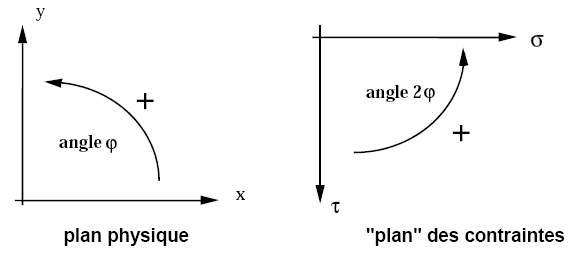
\includegraphics[scale=0.4]{ch2/image8.png}
    \captionof{figure}{Inversion du sens de l'axe $\tau$}
    \end{center}}\ \\
    
    Construisons dès à présent le cercle de Mohr connaissant l'état de contraite dans les axes $x$ et $y$.
    \begin{center}
    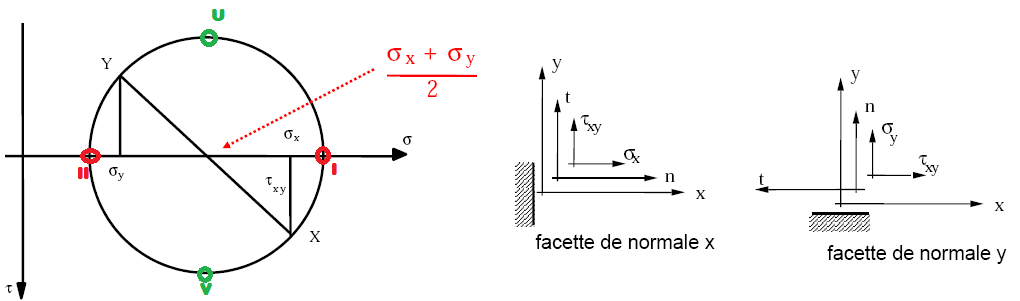
\includegraphics[scale=0.4]{ch2/image9.png}
    \captionof{figure}{Construction du cercle de Mohr}
    \end{center}   
    Sur le cercle de Mohr ci-dessus, le point représentatif (dans les axes locaux $n,t$ (axes des différentes
    facettes à droite du cercle)) $x$ est donné par $\sigma_x, \tau_{xy}$ et le point $y$ par $\sigma_y, 
    -\tau_{xy}$. Ceci défini, on obtient le fameux cercle : chaque point situé sur celui-ci donne l'information
    sur la composante normale et tangentielle du vecteur contrainte associée à la direction correspondante.\\
    
    \subsubsection{Rotation de 180 degrés}
    Si l'on venait à imposer une rotation de notre facette de $\pi$ radians, on se déplacerait de $2\pi$ radians sur le cercle
    de Mohr, c'est à dire le même point. Ceci est évident si l'on se rappelle que $\overline{T}^{(u)} =
    -\overline{T}^{(-u)}$.
    
    \subsubsection{Contraintes principales et direction principales}
    Par convention, $I$ est à droite et $II$ à gauche. Ces deux points montrent qu'il n'y a pas de contraintes
    tangentielles sur ces deux directions : il n'agit respectivement que $\sigma_1$ et $\sigma_2$.\\
    On peut directement obtenir les contraintes principales à partir du cercle de Mohr : La somme des 
    contraintes divisée par deux me place au centre du cercle, il me suffit d'appliquer pythagore :
    \begin{equation}
    \left.\begin{array}{c}
    \sigma_1\\
    \sigma_2
    \end{array}\right\} = \dfrac{\sigma_1+\sigma_2}{2}\pm \sqrt{\left(\dfrac{\sigma_1-\sigma_2}{2}\right)^2
    + \tau_{xy}^2}
    \end{equation}
    L'angle étant défini par la relation 
    \begin{equation}
    \tan 2\theta = \dfrac{2\tau_{xy}}{\sigma_x-\sigma_y}
    \end{equation}
    Attention tout de même à l'utilisation de cette formule pour le calcul de $\theta$. On a en effet, de 
    façon explicite
    \begin{equation}
    \theta = \frac{1}{2}\arctan\left(\dfrac{2\tau_{xy}}{\sigma_x-\sigma_y}\right) \pm k\dfrac{\pi}{2}
    \end{equation}
    où la valeur de $k$ est telle que $-\frac{\pi}{2} \leq \theta \leq \frac{\pi}{2}$ et $sign(\theta) =
    sign(\tau_{xy})$.
    
    \subsubsection{Contraintes tangentielle extrémum}
    Cette fois-ci, les points $U$ et $V$ sont les points ou se trouve la plus grande composante tangentielle.
    
    \subsubsection{Composantes après changement d'axe}
    \begin{wrapfigure}[7]{r}{5cm}
    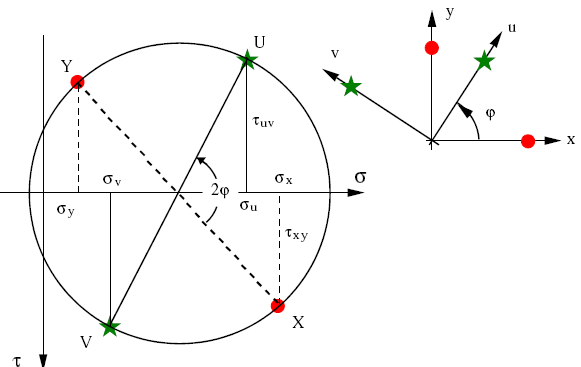
\includegraphics[scale=0.3]{ch2/image10.png}
    \captionof{figure}{Changement d'axes}
    \end{wrapfigure}
    Comment trouver les composantes apres un changement d'axe ? Les axes d'origines sont pointés par une boule
    rouge, et je suppose que mes composantes $\sigma_x$ et $\sigma_y$ m'amènent à cet endroit sur le cercle.\\
    
    Je trouve mes nouveaux axes (étoile verte) en faisant une rotation d'angle $\varphi$. Pour tenir en compte
    ce changement d'axe, il suffit de tourner d'un angle $2\varphi$.
    
    \subsubsection{Signe des contraintes tangentielles}

    Qu'est ce qui se passe quand $\varphi$ augmente légèrement ? Reprenons les relation analytiques :
    \begin{equation}
    \begin{array}{ll}
    \sigma_u &= \dfrac{\sigma_x+\sigma_y}{2} + \dfrac{\sigma_x-\sigma_y}{2}\cos 2\varphi + \tau_{xy}\sin
    2\varphi\\
    \tau_{uv} &= -\dfrac{\sigma_x-\sigma_y}{2}\sin 2\varphi + \tau_{xy}\cos 2\varphi
    \end{array}
    \end{equation}       
    On trouve, après ré-écriture que 
    \begin{equation}
    \frac{\partial \sigma_u}{\partial \varphi} = 2\tau_{uv}
    \end{equation}
    Soit les directions $I$ et $II$, ou je n'ai que des composantes normales. Si je suis sur l'axe $I$ et que
    j'augmente l'angle, la composante $\sigma$ ne peut que diminuer. Cela signifique que $\tau < 0$ et c'est
    pour ça qu'il pointe vers le bas : \textit{$\tau$ pointe toujours vers la direction de contrainte maximale.}
    \\ \textbf{Point de rayonnement ?}
    
    \subsubsection{Exemples}
    \begin{wrapfigure}[11]{l}{7cm}
    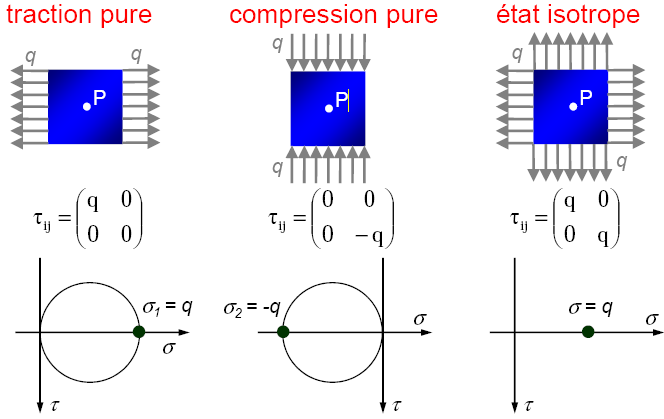
\includegraphics[scale=0.4]{ch2/image11.png}
    \captionof{figure}{Exemples de cercles de Mohr}
    \end{wrapfigure}
    Reprenons les trois exemples du slide 35 :
    
    \begin{itemize}
    \item En traction pure, je n'ai que $\sigma$, pas de composantes tangentielle.
    \item En compression pure, $\sigma_x=0$ de même que mes contraintes tangentielle. Par contre, $\sigma_y
    = -q$, car $q$ est toujours positif.
    \item Dans le cas isotrope, $\sigma_x = \sigma_y$ et le cercle de Mohr se réduit à un point. C'est, par
    exemple, la pression dans un fluide.
    \end{itemize}
    
